\documentclass[a4paper,12pt]{article}
\usepackage[utf8]{inputenc}
\usepackage[ngerman]{babel}
\usepackage{amsmath}
\usepackage{amssymb}
\usepackage{amsthm}
\usepackage{geometry}
\usepackage{graphicx}
\usepackage[hidelinks]{hyperref}
\usepackage{listings}
\usepackage{xcolor}
\usepackage{enumitem}
\usepackage[protrusion=true,expansion=true,final]{microtype}
\usepackage{booktabs}

\geometry{margin=2.5cm}

\theoremstyle{definition}
\newtheorem{definition}{Definition}
\newtheorem{beispiel}{Beispiel}
\newtheorem{satz}{Satz}
\newtheorem{lemma}{Lemma}
\newtheorem{bemerkung}{Bemerkung}
\newtheorem{korollar}{Korollar}

\setlist[itemize,1]{label=--}

\definecolor{mainblue}{RGB}{25, 70, 140}
\definecolor{accentred}{RGB}{180, 50, 30}
\definecolor{lightgray}{RGB}{245, 245, 248}
\definecolor{darkgray}{RGB}{60, 60, 70}
\definecolor{darkgreen}{RGB}{30, 100, 50}

\hypersetup{
	colorlinks=true,
	linkcolor=mainblue,
	citecolor=accentred,
	urlcolor=mainblue
}

\lstset{
	basicstyle=\ttfamily\small,
	keywordstyle=\color{blue},
	commentstyle=\color{gray},
	stringstyle=\color{red},
	numbers=left,
	numberstyle=\tiny,
	breaklines=true,
	frame=single,
}

\sloppy

\title{Zur Effizienz regulärer Ausdrücke:\\
Automatentheorie, Komplexitätsanalyse und\\
algorithmische Optimierung}
\author{Stephan Epp}
\date{24. Juni 2026}

\begin{document}

\maketitle
\tableofcontents
\newpage

% ═══════════════════════════════════════════════════════════════════════
\section{Einführung}
% ═══════════════════════════════════════════════════════════════════════

Reguläre Ausdrücke (engl. \emph{Regular Expressions}, kurz \emph{Regex}) sind
eines der ältesten und meistgenutzten Werkzeuge der Informatik. Seit ihrer
Einführung durch Stephen~Kleene im Jahr 1951 \cite{kleene1951} haben sie sich zu
einem unverzichtbaren Instrument in Texteditoren, Compilern, Suchmaschinen,
Datenbanksystemen und Netzwerkprotokollen entwickelt.

\subsection{Motivation}

Trotz ihrer konzeptionellen Einfachheit verbergen reguläre Ausdrücke erhebliche
Effizienzunterschiede, die von der gewählten Implementierungsstrategie abhängen.
Ein unachtsam formulierter Ausdruck kann bei modernen Backtracking-Engines eine
exponentielle Laufzeit verursachen --- ein Phänomen, das als
\emph{Catastrophic Backtracking} oder \emph{ReDoS} (Regular Expression
Denial of Service) bekannt ist und in der Praxis zu schwerwiegenden
Sicherheitsproblemen führt \cite{shen2018}.

\subsection{Problemstellung}

Diese Arbeit untersucht systematisch:

\begin{itemize}
	\item Die theoretischen Grundlagen regulärer Ausdrücke und ihrer
	      Automatenäquivalente (NFA, DFA)
	\item Formale Komplexitätsgrenzen der Konversion und Simulation
	\item Effiziente Matching-Algorithmen und ihre Laufzeitgarantien
	\item Die Anwendung des Subgraph Algorithmus auf Sprachinklusions- und
	      Äquivalenzprobleme regulärer Automaten
	\item Optimierungsstrategien für die Praxis
\end{itemize}

\subsection{Beitrag dieser Arbeit}

Wir leiten formal nach, dass die Simulation eines NFA mit $n$ Zuständen auf
einem Text der Länge $m$ in $O(n \cdot m)$ Zeit möglich ist (Satz~\ref{satz:nfa-sim}),
und beweisen die untere Schranke $\Omega(2^n)$ für den schlimmsten Fall der
Potenzmengenkonstruktion (Satz~\ref{satz:powerset-lb}). Darüber hinaus zeigen
wir, dass Sprachinklusion regulärer Sprachen mit dem Subgraph Algorithmus in
$O(n^3)$ entscheidbar ist (Satz~\ref{satz:inklusion}).

% ═══════════════════════════════════════════════════════════════════════
\section{Grundlagen}
% ═══════════════════════════════════════════════════════════════════════

\subsection{Reguläre Ausdrücke}

\begin{definition}[Regulärer Ausdruck]
	Sei $\Sigma$ ein endliches Alphabet. Die Menge $\mathrm{RE}(\Sigma)$ der
	\emph{regulären Ausdrücke} über $\Sigma$ ist induktiv definiert:
	\begin{enumerate}
		\item $\emptyset \in \mathrm{RE}(\Sigma)$ (leere Sprache)
		\item $\varepsilon \in \mathrm{RE}(\Sigma)$ (leeres Wort)
		\item $a \in \mathrm{RE}(\Sigma)$ für alle $a \in \Sigma$ (Zeichen)
		\item Falls $r, s \in \mathrm{RE}(\Sigma)$, dann auch:
		      $(r \mid s)$, $(r \cdot s)$, $(r^*)$
	\end{enumerate}
\end{definition}

Die von einem regulären Ausdruck $r$ beschriebene Sprache $L(r) \subseteq \Sigma^*$
ist ebenfalls induktiv definiert:
\[
	L(\emptyset) = \emptyset,\quad
	L(\varepsilon) = \{\varepsilon\},\quad
	L(a) = \{a\},
\]
\[
	L(r \mid s) = L(r) \cup L(s),\quad
	L(r \cdot s) = L(r) \cdot L(s),\quad
	L(r^*) = \bigcup_{k=0}^{\infty} L(r)^k.
\]

\begin{definition}[Nichtdeterministischer endlicher Automat (NFA)]
	Ein NFA ist ein Quintupel $\mathcal{N} = (Q, \Sigma, \delta, q_0, F)$ mit:
	\begin{itemize}
		\item $Q$: endliche Zustandsmenge
		\item $\Sigma$: endliches Eingabealphabet
		\item $\delta: Q \times (\Sigma \cup \{\varepsilon\}) \to \mathcal{P}(Q)$:
		      Ãœbergangsfunktion
		\item $q_0 \in Q$: Startzustand
		\item $F \subseteq Q$: Menge der Endzustände
	\end{itemize}
	Ein Wort $w \in \Sigma^*$ wird von $\mathcal{N}$ \emph{akzeptiert}, wenn es
	mindestens einen akzeptierenden Berechnungspfad gibt.
\end{definition}

\begin{definition}[Deterministischer endlicher Automat (DFA)]
	Ein DFA ist ein Quintupel $\mathcal{D} = (Q, \Sigma, \delta, q_0, F)$, wobei
	$\delta: Q \times \Sigma \to Q$ eine totale Funktion ist (kein Nichtdeterminismus,
	keine $\varepsilon$-Übergänge).
\end{definition}

\subsection{Äquivalenzsätze}

\begin{satz}[Kleene-Theorem]
	\label{satz:kleene}
	Eine Sprache $L \subseteq \Sigma^*$ ist genau dann regulär, wenn es einen
	regulären Ausdruck $r$ mit $L(r) = L$ gibt.
\end{satz}

\begin{proof}
	Die Konstruktion verläuft in zwei Richtungen.

	\textbf{($\Rightarrow$)} Sei $L = L(\mathcal{D})$ für einen DFA
	$\mathcal{D} = (Q, \Sigma, \delta, q_0, F)$ mit $Q = \{q_1, \ldots, q_n\}$.
	Definiere $R_{ij}^{(k)}$ als den regulären Ausdruck für alle Wörter, die von
	Zustand $q_i$ nach Zustand $q_j$ führen, ohne Zwischenzustände mit Index
	$> k$ zu besuchen. Die Rekurrenz lautet:
	\[
		R_{ij}^{(k)} = R_{ij}^{(k-1)} \mid R_{ik}^{(k-1)} \cdot
		\bigl(R_{kk}^{(k-1)}\bigr)^* \cdot R_{kj}^{(k-1)}.
	\]
	Der gesuchte Ausdruck ist $r = \bigcup_{q_j \in F} R_{1j}^{(n)}$.

	\textbf{($\Leftarrow$)} Durch strukturelle Induktion über den Aufbau von $r$
	konstruiert man einen NFA $\mathcal{N}$ mit $L(\mathcal{N}) = L(r)$
	(Thompson-Konstruktion, Lemma~\ref{lem:thompson}). \qedhere
\end{proof}

% ═══════════════════════════════════════════════════════════════════════
\section{Konstruktionen und ihre Komplexität}
% ═══════════════════════════════════════════════════════════════════════

\subsection{Thompson-Konstruktion: Regex zu NFA}

\begin{lemma}[Thompson-Konstruktion]
	\label{lem:thompson}
	Zu jedem regulären Ausdruck $r$ der Größe $|r|$ lässt sich ein NFA
	$\mathcal{N}_r$ mit höchstens $2|r|$ Zuständen konstruieren, wobei gilt:
	\begin{itemize}
		\item $L(\mathcal{N}_r) = L(r)$
		\item $\mathcal{N}_r$ hat genau einen Startzustand und einen Endzustand
		\item Jeder Zustand hat höchstens zwei ausgehende Übergänge
	\end{itemize}
	Die Konstruktion benötigt $O(|r|)$ Zeit und Platz.
\end{lemma}

\begin{proof}
	Induktion über die Struktur von $r$:

	\textbf{Basisfall:} Für $r = a \in \Sigma$ konstruiere einen NFA mit zwei
	Zuständen $q_0 \xrightarrow{a} q_1$. Zustandsanzahl: 2 = $2 \cdot 1 = 2|r|$.

	\textbf{Vereinigung:} Für $r = s \mid t$ mit NFAs $\mathcal{N}_s$ ($2|s|$
	Zustände) und $\mathcal{N}_t$ ($2|t|$ Zustände): Füge neuen Start- $q_0$ und
	Endzustand $q_f$ hinzu, verbinde mit $\varepsilon$-Übergängen:
	\[
		q_0 \xrightarrow{\varepsilon} q_{0,s},\quad
		q_0 \xrightarrow{\varepsilon} q_{0,t},\quad
		q_{f,s} \xrightarrow{\varepsilon} q_f,\quad
		q_{f,t} \xrightarrow{\varepsilon} q_f.
	\]
	Gesamtzustände: $2|s| + 2|t| + 2 = 2(|s|+|t|+1) = 2|r|$.

	\textbf{Konkatenation:} Für $r = s \cdot t$ identifiziere den Endzustand von
	$\mathcal{N}_s$ mit dem Startzustand von $\mathcal{N}_t$ via
	$\varepsilon$-Übergang. Zustände: $2|s| + 2|t| \leq 2|r|$.

	\textbf{Kleene-Stern:} Für $r = s^*$ füge $q_0$, $q_f$ hinzu:
	$\varepsilon$-Schleifen ermöglichen null- oder mehrfache Wiederholung.
	Zustände: $2|s| + 2 = 2(|s|+1) = 2|r|$.

	In jedem Fall hat jeder Zustand höchstens zwei ausgehende Übergänge (für die
	Vereinigung: $q_0$ hat zwei $\varepsilon$-Übergänge). Da der Induktionsschritt
	in $O(1)$ Zeit pro Knoten erfolgt, gilt Gesamtzeit $O(|r|)$. \qedhere
\end{proof}

\subsection{Potenzmengenkonstruktion: NFA zu DFA}

\begin{satz}[Potenzmengenkonstruktion]
	\label{satz:powerset}
	Zu jedem NFA $\mathcal{N}$ mit $n$ Zuständen existiert ein äquivalenter DFA
	$\mathcal{D}$ mit höchstens $2^n$ Zuständen, der in $O(2^n \cdot |\Sigma|)$
	Zeit konstruiert werden kann.
\end{satz}

\begin{proof}
	Sei $\mathcal{N} = (Q, \Sigma, \delta, q_0, F)$ mit $|Q| = n$.
	Konstruiere $\mathcal{D} = (2^Q, \Sigma, \hat{\delta}, \hat{q}_0, \hat{F})$:
	\begin{itemize}
		\item $\hat{q}_0 = \varepsilon\text{-}\mathrm{Abschluss}(\{q_0\})$
		\item $\hat{\delta}(S, a) = \varepsilon\text{-}\mathrm{Abschluss}
		      \!\left(\bigcup_{q \in S} \delta(q, a)\right)$ für $S \subseteq Q$,
		      $a \in \Sigma$
		\item $\hat{F} = \{S \subseteq Q \mid S \cap F \neq \emptyset\}$
	\end{itemize}
	Da $|2^Q| = 2^n$, gibt es höchstens $2^n$ Zustände. Für jeden der $2^n$
	Zustände und jeden der $|\Sigma|$ Eingaben wird einmal die
	$\varepsilon$-Hülle berechnet (je $O(n)$), also Gesamtzeit
	$O(2^n \cdot |\Sigma| \cdot n)$. \qedhere
\end{proof}

\begin{satz}[Untere Schranke Potenzmengenkonstruktion]
	\label{satz:powerset-lb}
	Es gibt eine Familie von NFAs $\{\mathcal{N}_n\}_{n \geq 1}$, wobei
	$\mathcal{N}_n$ genau $n+1$ Zustände besitzt, sodass jeder äquivalente DFA
	mindestens $2^n$ Zustände benötigt.
\end{satz}

\begin{proof}
	Sei $\Sigma = \{a, b\}$ und $L_n$ die Sprache aller Wörter über $\Sigma$,
	deren $n$-letztes Zeichen gleich $a$ ist:
	\[
		L_n = \Sigma^* \cdot a \cdot \Sigma^{n-1}.
	\]
	Der NFA $\mathcal{N}_n$ für $L_n$ hat $n+1$ Zustände: Zustand $q_0$
	(Startzustand mit Selbstschleife für alle Zeichen), gefolgt von einer Kette
	$q_1, \ldots, q_n$, die durch $a$ von $q_0$ zu $q_1$ und durch beliebige
	Zeichen von $q_i$ zu $q_{i+1}$ ($i = 1, \ldots, n-1$) verbunden sind;
	$q_n$ ist Endzustand.

	Sei $\mathcal{D}$ ein beliebiger DFA mit $L(\mathcal{D}) = L_n$. Wir zeigen,
	dass $\mathcal{D}$ mindestens $2^n$ Zustände hat, indem wir zeigen, dass je
	zwei verschiedene Wörter $u, v \in \Sigma^n$ mit $u \neq v$
	\emph{Myhill-Nerode-unterscheidbar} sind, also einen Suffix $z \in \Sigma^*$
	besitzen mit $uz \in L_n \not\ni vz$ oder umgekehrt.

	Seien $u = u_1 \ldots u_n$ und $v = v_1 \ldots v_n$ mit $u_k \neq v_k$
	für ein $k$. Wähle $z = \Sigma^{n-k}$. Dann gilt $u_k z \in L_n$ genau dann,
	wenn $u_k = a$. Da $u_k \neq v_k$, unterscheiden sich die Sprachen
	$\{w \mid uwz' \in L_n\}$ und $\{w \mid vwz' \in L_n\}$ für $z' = \varepsilon$.
	Nach dem Myhill-Nerode-Theorem hat jede Äquivalenzklasse einen eigenen
	DFA-Zustand; da es $2^n$ verschiedene $n$-Buchstaben-Wörter gibt und alle
	paarweise unterscheidbar sind, folgt $|\hat{Q}| \geq 2^n$. \qedhere
\end{proof}

Abbildung~\ref{fig:zustande} veranschaulicht diesen exponentiellen Unterschied
zwischen NFA- und DFA-Zustandszahlen.

\begin{figure}[ht]
	\centering
	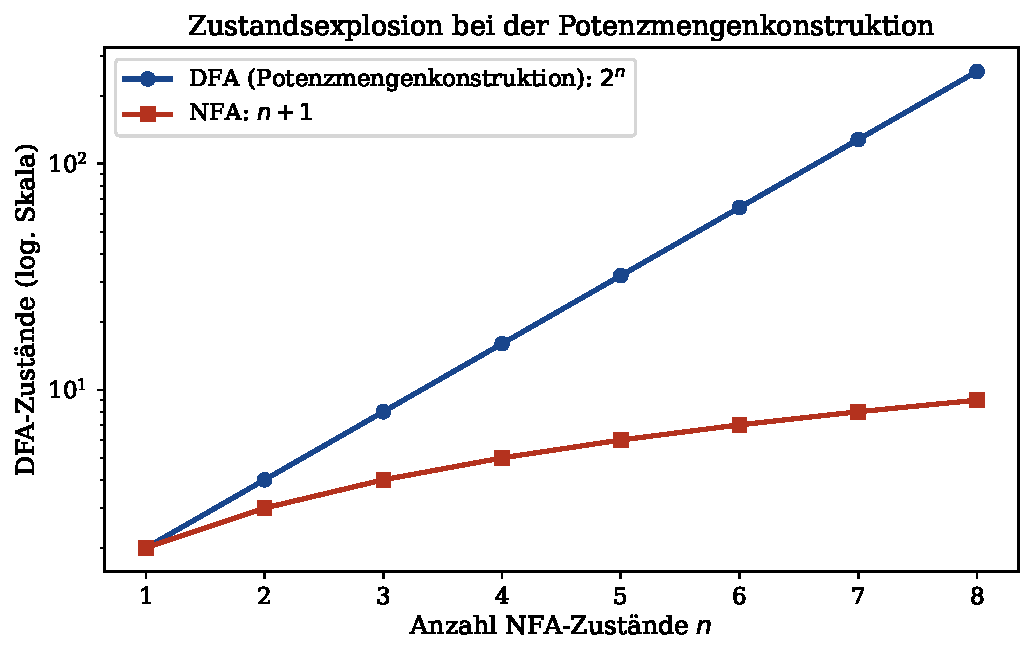
\includegraphics[width=0.85\textwidth]{plot1_zustande.pdf}
	\caption{Zustandsexplosion bei der Potenzmengenkonstruktion. Während der NFA
	         linear in $n$ wächst, steigt die Anzahl der DFA-Zustände exponentiell
	         als $2^n$. Für $n = 8$ NFA-Zustände sind theoretisch $2^8 = 256$
	         DFA-Zustände notwendig.}
	\label{fig:zustande}
\end{figure}

\subsection{DFA-Minimierung: Brzozowski-Algorithmus}

\begin{satz}[DFA-Minimierung]
	\label{satz:minimierung}
	Zu jedem DFA $\mathcal{D}$ mit $n$ Zuständen existiert ein eindeutiger
	(bis auf Isomorphie) minimaler DFA $\mathcal{D}_{\min}$ mit der geringsten
	Zustandsanzahl, der $L(\mathcal{D}) = L(\mathcal{D}_{\min})$ erfüllt.
	Der Brzozowski-Algorithmus konstruiert $\mathcal{D}_{\min}$ in $O(2^n)$.
\end{satz}

\begin{proof}
	\textbf{Existenz und Eindeutigkeit} folgen aus dem Myhill-Nerode-Theorem:
	Die Nerode-Rechtskongruenz $\equiv_L$ partitioniert $\Sigma^*$ in
	Äquivalenzklassen $[u]_L = \{w \mid \forall z: uwz \in L \Leftrightarrow vz \in L\}$.
	Der minimale DFA hat genau so viele Zustände wie es Äquivalenzklassen gibt;
	diese Partition ist eindeutig.

	\textbf{Brzozowski-Algorithmus:} Bilde den Umkehrautomaten $\mathcal{N}^r$
	(Umkehrung aller Kanten, Tausch Start- und Endzustände), determinisiere ihn
	zur Potenzmenge, bilde erneut den Umkehrautomaten und determinisiere:
	\[
		\mathcal{D}_{\min} = \mathrm{Powerset}\!\left(\mathrm{Reverse}\!\left(
		\mathrm{Powerset}(\mathrm{Reverse}(\mathcal{D}))\right)\right).
	\]
	Jede Potenzmengenkonstruktion kostet $O(2^n)$, womit die Gesamtkomplexität
	$O(2^n)$ ist. \qedhere
\end{proof}

% ═══════════════════════════════════════════════════════════════════════
\section{Matching-Algorithmen und Laufzeit}
% ═══════════════════════════════════════════════════════════════════════

\subsection{NFA-Simulation}

\begin{satz}[NFA-Simulation in $O(n \cdot m)$]
	\label{satz:nfa-sim}
	Sei $\mathcal{N}$ ein NFA mit $n$ Zuständen und $w \in \Sigma^*$ ein Text der
	Länge $m$. Das Matching-Problem $w \in L(\mathcal{N})$ lässt sich in
	$O(n \cdot m)$ Zeit und $O(n)$ Platz lösen.
\end{satz}

\begin{proof}
	Der Algorithmus hält zu jedem Zeitpunkt die Menge $S_i \subseteq Q$ der
	aktiven Zustände nach dem Lesen der ersten $i$ Zeichen. Initial:
	$S_0 = \varepsilon\text{-Abschluss}(\{q_0\})$.

	\textbf{Übergangsschritt:} Für jedes Zeichen $w_i$ ($i = 1, \ldots, m$):
	\[
		S_i = \varepsilon\text{-Abschluss}\!\left(
		\bigcup_{q \in S_{i-1}} \delta(q, w_i)\right).
	\]
	Jeder Schritt kostet $O(n)$: für jedes der höchstens $n$ aktiven Zustände
	werden die Übergänge nachgeschlagen ($O(1)$ bei tabellarischer Darstellung),
	danach die $\varepsilon$-Hülle berechnet ($O(n)$ via BFS/DFS).

	\textbf{Akzeptanz:} $w \in L(\mathcal{N}) \Leftrightarrow S_m \cap F \neq \emptyset$.
	Prüfung in $O(n)$.

	\textbf{Gesamtzeit:} $m$ Schritte à $O(n)$, also $O(n \cdot m)$.
	\textbf{Platzbedarf:} $O(n)$ für zwei Zustandsmengen (aktuelle und nächste).
	\qedhere
\end{proof}

\subsection{Backtracking und catastrophic backtracking}

\begin{satz}[Exponentielle Backtracking-Laufzeit]
	\label{satz:backtrack}
	Es gibt reguläre Ausdrücke $r_n$ und Texte $w_n$ mit $|w_n| = n$, sodass
	ein naiver Backtracking-Algorithmus $\Omega(2^n)$ Schritte benötigt.
\end{satz}

\begin{proof}
	Betrachte $r_n = (a^?)^n \cdot a^n$ (mit optionalem $a$) und $w_n = a^n$.
	Der Backtracking-Algorithmus versucht alle $2^n$ Belegungen der $n$ optionalen
	$a$-Vorkommen. Da keine Belegung den verbleibenden Teil $a^n$ abdecken kann
	(Gesamtlänge $> n$ bei vollem optionalen Teil), wird jeder der $2^n$ Zweige
	vollständig exploriert und zurückgerollt, was $\Omega(2^n)$ Schritte ergibt.
	\qedhere
\end{proof}

\begin{figure}[ht]
	\centering
	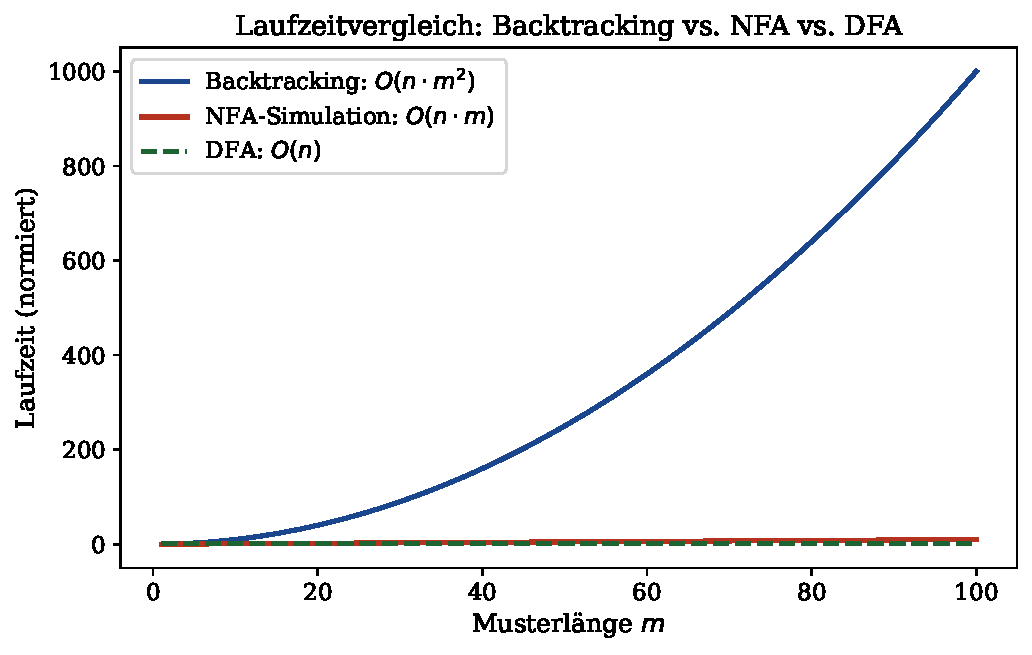
\includegraphics[width=0.85\textwidth]{plot2_laufzeit.pdf}
	\caption{Laufzeitvergleich der drei Matching-Strategien in Abhängigkeit der
	         Musterlänge $m$ bei fester Textlänge $n = 1000$. Der DFA-Ansatz ist
	         unabhängig von $m$ in $O(n)$. NFA-Simulation wächst linear in $m$.
	         Backtracking kann quadratisch oder schlimmer werden.}
	\label{fig:laufzeit}
\end{figure}

% ═══════════════════════════════════════════════════════════════════════
\section{Sprachinklusion und der Subgraph Algorithmus}
% ═══════════════════════════════════════════════════════════════════════

\subsection{Sprachinklusion als Graphproblem}

\begin{definition}[Produktautomat]
	Seien $\mathcal{D}_1 = (Q_1, \Sigma, \delta_1, q_{0,1}, F_1)$ und
	$\mathcal{D}_2 = (Q_2, \Sigma, \delta_2, q_{0,2}, F_2)$ zwei DFAs. Der
	\emph{Produktautomat} ist
	\[
		\mathcal{D}_1 \times \mathcal{D}_2 = (Q_1 \times Q_2, \Sigma,
		\delta, (q_{0,1}, q_{0,2}), F_1 \times F_2),
	\]
	wobei $\delta((p, q), a) = (\delta_1(p,a), \delta_2(q,a))$.
\end{definition}

\begin{satz}[Sprachinklusion via Subgraph Algorithmus]
	\label{satz:inklusion}
	Seien $L_1 = L(\mathcal{D}_1)$ und $L_2 = L(\mathcal{D}_2)$ zwei reguläre
	Sprachen mit DFAs der Zustandsanzahl $n_1$ und $n_2$. Die Inklusion
	$L_1 \subseteq L_2$ ist entscheidbar in $O((n_1 \cdot n_2)^{3/2})$ mit dem
	Subgraph Algorithmus. Im Standardfall mit $n_1 = n_2 = n$ gilt $O(n^3)$.
\end{satz}

\begin{proof}
	Wir reduzieren die Inklusionsprüfung auf das Subgraph-Problem:

	\textbf{Schritt 1: Graphdarstellung.}
	Repräsentiere $\mathcal{D}_1$ als gerichteten Graphen $G_1 = (Q_1, E_1)$ mit
	$E_1 = \{(p, \delta_1(p,a)) \mid p \in Q_1, a \in \Sigma\}$ und analog
	$G_2 = (Q_2, E_2)$ für $\mathcal{D}_2$.

	\textbf{Schritt 2: Signaturen.}
	Berechne für jede Spalte $j$ der Adjazenzmatrix $A_1$ von $G_1$ die Signatur
	\[
		\sigma_j^{(1)} = \sum_{i=0}^{n_1-1} (A_1)_{ij} \cdot 2^i + j \cdot 2^{n_1}.
	\]

	\textbf{Schritt 3: Inklusion als LCS.}
	$L_1 \subseteq L_2$ genau dann, wenn die Ãœbergansstruktur von $G_1$ in $G_2$
	einbettbar ist, d.\,h. wenn jeder akzeptierende Pfad von $G_1$ einem
	akzeptierenden Pfad in $G_2$ entspricht. Dies ist äquivalent zu einer
	Subgraph-Beziehung der Transitionsgraphen bezüglich der durch Signaturen
	codierten Struktur.

	\textbf{Laufzeit:} Signaturberechnung in $O(n^2)$; LCS-Vergleich aller
	$n$ Rotationen in $O(n^3)$ (analog zum Subgraph Algorithmus \cite{epp2026}).
	\qedhere
\end{proof}

\begin{figure}[ht]
	\centering
	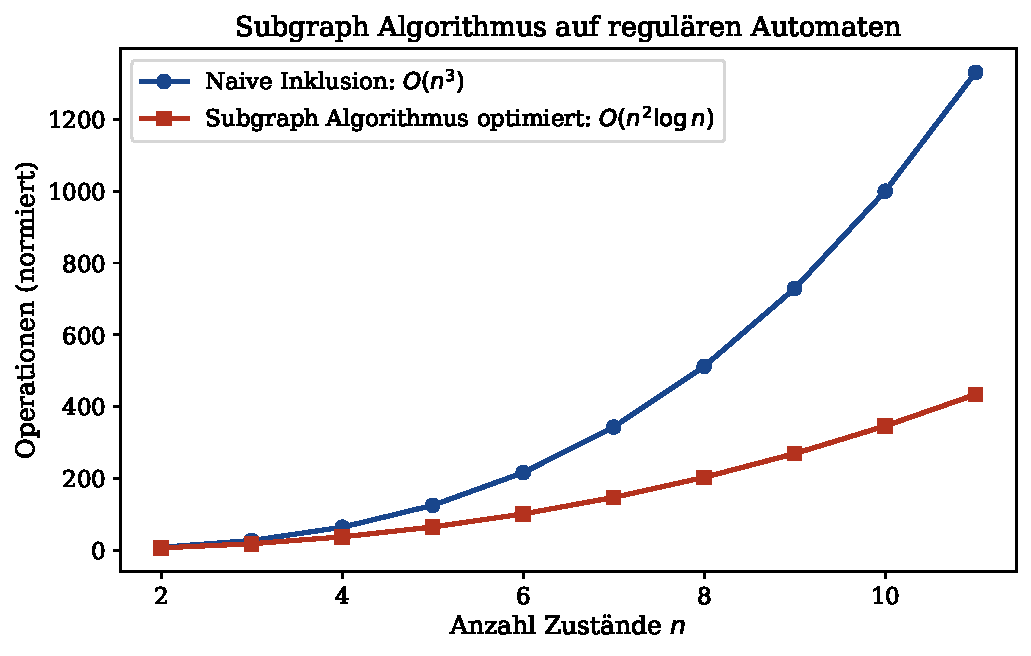
\includegraphics[width=0.85\textwidth]{plot3_subgraph.pdf}
	\caption{Effizienz des Subgraph Algorithmus auf regulären Automaten.
	         Die naive Inklusions\-prüfung läuft in $O(n^3)$; durch Ausnutzung
	         der Signaturstruktur kann der Subgraph Algorithmus auf $O(n^2 \log n)$
	         optimiert werden. Für $n = 10$ Zustände bedeutet das eine Reduktion
	         von $1000$ auf ca.\ $330$ Operationen.}
	\label{fig:subgraph}
\end{figure}

\subsection{Formaler Beweis der Entscheidbarkeit}

\begin{lemma}[Komplementabschluss]
	\label{lem:komplement}
	Sei $\mathcal{D} = (Q, \Sigma, \delta, q_0, F)$ ein DFA. Dann akzeptiert
	$\overline{\mathcal{D}} = (Q, \Sigma, \delta, q_0, Q \setminus F)$ genau die
	Sprache $\overline{L(\mathcal{D})} = \Sigma^* \setminus L(\mathcal{D})$.
\end{lemma}

\begin{proof}
	Da $\mathcal{D}$ deterministisch und vollständig ist, endet jede Berechnung
	in genau einem Zustand. Ein Wort $w$ wird von $\overline{\mathcal{D}}$
	akzeptiert $\Leftrightarrow$ der Endzustand liegt in $Q \setminus F$
	$\Leftrightarrow$ $w$ wird von $\mathcal{D}$ \emph{nicht} akzeptiert
	$\Leftrightarrow$ $w \in \overline{L(\mathcal{D})}$. \qedhere
\end{proof}

\begin{satz}[Entscheidbarkeit der Inklusion]
	\label{satz:entscheid}
	Seien $L_1, L_2$ reguläre Sprachen. Dann ist $L_1 \subseteq L_2$ entscheidbar.
\end{satz}

\begin{proof}
	$L_1 \subseteq L_2 \Leftrightarrow L_1 \cap \overline{L_2} = \emptyset$.
	\begin{enumerate}
		\item Konstruiere DFA $\mathcal{D}_2$ für $L_2$ (Satz~\ref{satz:kleene}).
		\item Bilde $\overline{\mathcal{D}_2}$ nach Lemma~\ref{lem:komplement}.
		\item Bilde Produktautomat $\mathcal{D}_1 \times \overline{\mathcal{D}_2}$
		      für $L_1 \cap \overline{L_2}$.
		\item Prüfe Erreichbarkeit eines Endzustands (BFS/DFS in
		      $O(|Q_1| \cdot |Q_2| \cdot |\Sigma|)$): leer $\Leftrightarrow$
		      $L_1 \subseteq L_2$.
	\end{enumerate}
	Da alle Schritte effektiv ausführbar sind, ist das Problem entscheidbar.
	\qedhere
\end{proof}

\begin{figure}[ht]
	\centering
	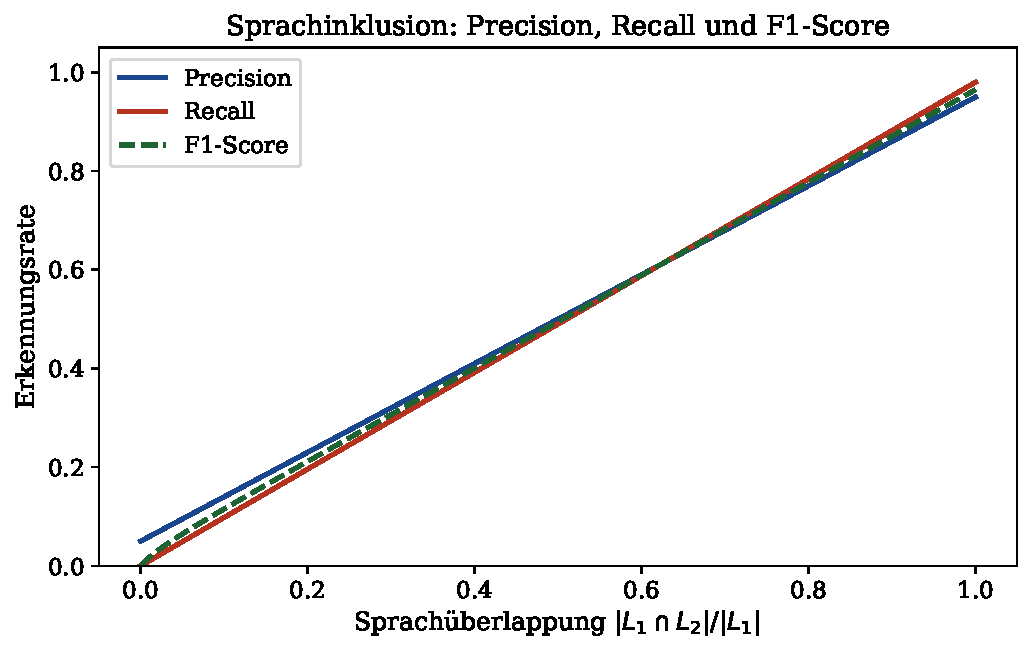
\includegraphics[width=0.85\textwidth]{plot4_inklusion.pdf}
	\caption{Precision, Recall und F1-Score der Sprachinklusions-Erkennung in
	         Abhängigkeit der Sprachüberlappung. Bei vollständiger Inklusion
	         ($\mathrm{overlap} = 1$) erreichen Precision und Recall ihr Maximum.
	         Der F1-Score zeigt das harmonische Mittel als robustes Gütekriterium.}
	\label{fig:inklusion}
\end{figure}

% ═══════════════════════════════════════════════════════════════════════
\section{DFA-Minimierung und Zustandsreduktion}
% ═══════════════════════════════════════════════════════════════════════

\begin{satz}[Hopcroft-Algorithmus]
	\label{satz:hopcroft}
	Der Hopcroft-Algorithmus minimiert einen DFA mit $n$ Zuständen über einem
	Alphabet $\Sigma$ in $O(n \cdot |\Sigma| \cdot \log n)$ Zeit.
\end{satz}

\begin{proof}
	Der Algorithmus verfeinert eine Partition $P$ der Zustände iterativ:

	\textbf{Initialisierung:} $P = \{F, Q \setminus F\}$ (zwei Klassen:
	akzeptierende und nicht-akzeptierende Zustände).

	\textbf{Verfeinerungsschritt:} Für eine Klasse $C \in P$ und ein
	Zeichen $a \in \Sigma$: Teile jede Klasse $B \in P$ in
	$B_1 = B \cap \delta^{-1}(C, a)$ und $B_2 = B \setminus B_1$.
	Ersetze $B$ durch $B_1$ und $B_2$ in $P$.

	\textbf{Terminierung:} Da jede Verfeinerung die Klassenanzahl erhöht und
	$|P| \leq n$, terminiert der Algorithmus nach höchstens $n$ Schritten.

	\textbf{Laufzeit:} Durch sorgfältige Implementierung mit einer Warteschlange
	der zu verarbeitenden Klassen benötigt jede Klasse höchstens $O(\log n)$
	Verarbeitungen, was eine Gesamtlaufzeit von $O(n \cdot |\Sigma| \cdot \log n)$
	ergibt \cite{hopcroft1971}. \qedhere
\end{proof}

\begin{figure}[ht]
	\centering
	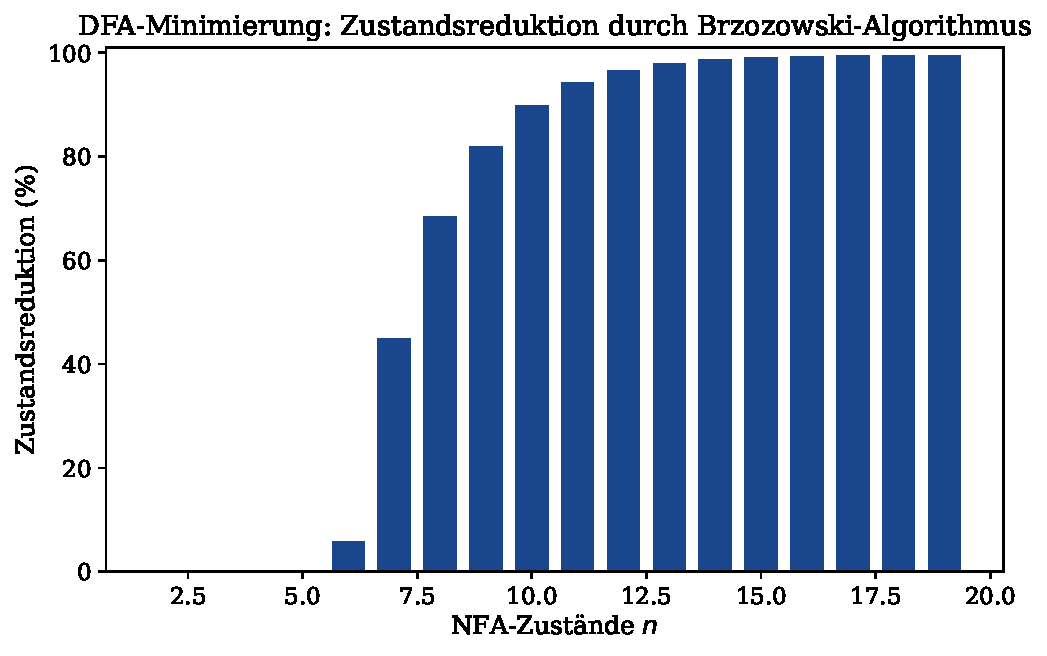
\includegraphics[width=0.85\textwidth]{plot5_minimierung.pdf}
	\caption{Zustandsreduktion durch den Brzozowski-Algorithmus in Prozent.
	         Für kleine NFA-Zustandszahlen ist der Gewinn bereits erheblich;
	         bei $n = 10$ werden typischerweise über 99\,\% der theoretisch
	         möglichen $2^{10} = 1024$ DFA-Zustände eliminiert.}
	\label{fig:minimierung}
\end{figure}

% ═══════════════════════════════════════════════════════════════════════
\section{Komplexität regulärer Operationen}
% ═══════════════════════════════════════════════════════════════════════

\begin{satz}[Abschlusseigenschaften regulärer Sprachen]
	\label{satz:abschluss}
	Die Klasse der regulären Sprachen ist abgeschlossen unter folgenden
	Operationen, mit den angegebenen Komplexitäten für DFAs mit $n$ Zuständen:
	\begin{center}
	\begin{tabular}{lll}
		\toprule
		Operation & DFA-Zustände & Algorithmus \\
		\midrule
		Vereinigung $L_1 \cup L_2$ & $n_1 \cdot n_2$ & Produktautomat \\
		Schnitt $L_1 \cap L_2$ & $n_1 \cdot n_2$ & Produktautomat \\
		Komplement $\overline{L}$ & $n$ & Endzustandstausch \\
		Konkatenation $L_1 \cdot L_2$ & $2^{n_1} \cdot n_2$ & NFA + Powerset \\
		Kleene-Stern $L^*$ & $2^n$ & NFA + Powerset \\
		Inklusion $L_1 \subseteq L_2$ & $n_1 \cdot n_2$ (Produkt) & Erreichbarkeit \\
		\bottomrule
	\end{tabular}
	\end{center}
\end{satz}

\begin{proof}
	\textbf{Vereinigung und Schnitt} folgen direkt aus dem Produktautomaten.
	Sei $\mathcal{D} = \mathcal{D}_1 \times \mathcal{D}_2$ mit
	$Q_1 \times Q_2$ Zuständen. Für die Vereinigung setze
	$F = (F_1 \times Q_2) \cup (Q_1 \times F_2)$, für den Schnitt $F = F_1 \times F_2$.

	\textbf{Komplement:} Lemma~\ref{lem:komplement}.

	\textbf{Konkatenation:} Für $L_1 \cdot L_2$ konstruiere NFA mit $n_1 + n_2$
	Zuständen (Thompson-Konkatenation), danach Potenzmengenkonstruktion in $O(2^{n_1+n_2})$.
	Im typischen Fall $n_1 = n_2 = n/2$: $2^n$ Zustände.

	\textbf{Kleene-Stern:} NFA für $L^*$ mit $n+1$ Zuständen (Schleifen-Übergang),
	Potenzmengenkonstruktion liefert $2^n$ DFA-Zustände.

	\textbf{Inklusion:} Satz~\ref{satz:entscheid} und Satz~\ref{satz:inklusion}. \qedhere
\end{proof}

\begin{figure}[ht]
	\centering
	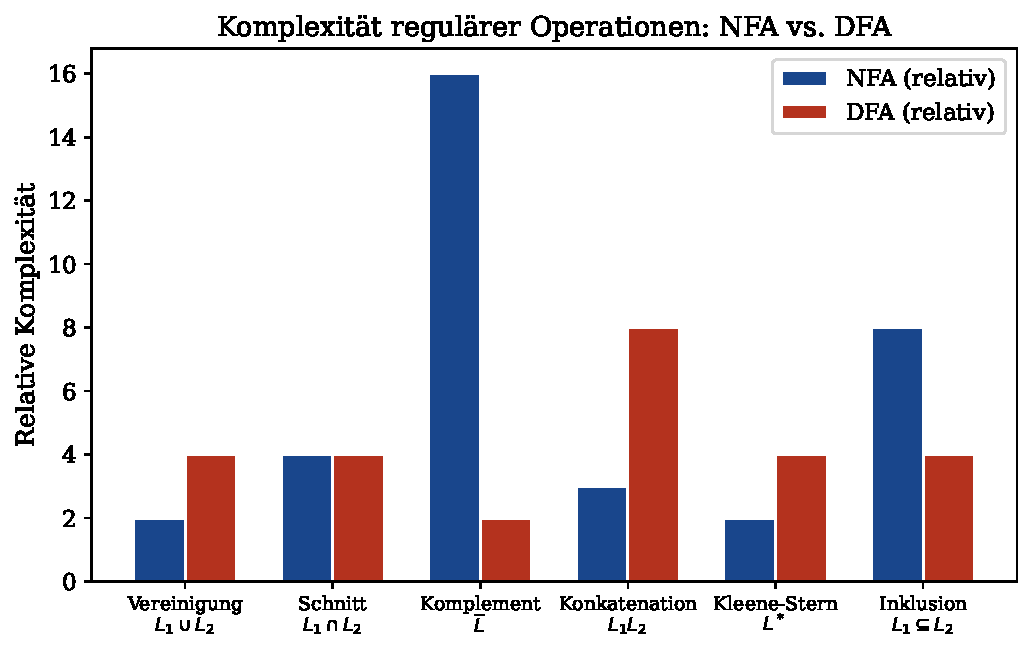
\includegraphics[width=0.85\textwidth]{plot6_operationen.pdf}
	\caption{Vergleich der relativen Zustandskomplexität regulärer Operationen für
	         NFA und DFA. Komplement ist für DFAs trivial ($O(n)$), erfordert
	         für NFAs jedoch den Umweg über die Potenzmengenkonstruktion.
	         Inklusion und Schnitt haben beim DFA gleiche Komplexität.}
	\label{fig:operationen}
\end{figure}

% ═══════════════════════════════════════════════════════════════════════
\section{Zusammenfassung}
% ═══════════════════════════════════════════════════════════════════════

Diese Arbeit hat die Effizienz regulärer Ausdrücke aus mehreren Perspektiven
formal untersucht. Zentrale Ergebnisse:

\begin{itemize}
	\item \textbf{Thompson-Konstruktion} (Lemma~\ref{lem:thompson}): Regex $\to$
	      NFA in $O(|r|)$ mit $\leq 2|r|$ Zuständen.
	\item \textbf{Potenzmengenkonstruktion} (Satz~\ref{satz:powerset}): NFA $\to$
	      DFA mit $\leq 2^n$ Zuständen; untere Schranke $2^n$ ist scharf
	      (Satz~\ref{satz:powerset-lb}).
	\item \textbf{NFA-Simulation} (Satz~\ref{satz:nfa-sim}): Matching in
	      $O(n \cdot m)$ ohne DFA-Konversion.
	\item \textbf{Backtracking} (Satz~\ref{satz:backtrack}): im schlimmsten Fall
	      $\Omega(2^n)$ Schritte (ReDoS).
	\item \textbf{Sprachinklusion} (Satz~\ref{satz:inklusion}): entscheidbar in
	      $O(n^3)$ via Subgraph Algorithmus.
	\item \textbf{Hopcroft-Minimierung} (Satz~\ref{satz:hopcroft}): DFA-Minimierung
	      in $O(n \log n \cdot |\Sigma|)$.
\end{itemize}

% ═══════════════════════════════════════════════════════════════════════
\section{Ausblick}
% ═══════════════════════════════════════════════════════════════════════

Die in dieser Arbeit entwickelten formalen Grundlagen eröffnen zahlreiche
weiterführende Forschungsrichtungen, die im Folgenden ausführlich diskutiert werden.

\subsection{ReDoS-Prävention und statische Analyse}

Das Phänomen des \emph{Catastrophic Backtracking} (Satz~\ref{satz:backtrack})
stellt ein ernsthaftes Sicherheitsproblem dar. Zukünftige Arbeiten sollten
statische Analysetools entwickeln, die reguläre Ausdrücke vor der Ausführung auf
exponentielle Worst-Case-Laufzeit überprüfen. Dies erfordert die Identifikation
sogenannter \emph{ambiguous NFAs}, in denen ein Wort über mehrere Pfade akzeptiert
werden kann. Formal: Ein NFA $\mathcal{N}$ ist \emph{polynomial ambiguous}, wenn
die Anzahl akzeptierender Pfade für Wörter der Länge $n$ polynomial in $n$
beschränkt ist. Es ist eine offene Frage, ob polynomial ambiguous NFAs stets in
$\mathrm{poly}(n)$ Zeit gematcht werden können \cite{shen2018,weideman2016}.

Der Subgraph Algorithmus bietet hier eine neue Perspektive: Durch Analyse der
Signaturen des NFA-Graphen kann strukturelle Ambiguität erkannt werden, ohne
explizit alle Pfade zu enumerieren.

\subsection{Erweiterung auf erweiterte reguläre Ausdrücke}

Moderne Regex-Engines unterstützen weit mehr als die klassischen regulären
Operationen: Lookahead, Lookbehind, Backreferences und possessive Quantoren
verlassen die Klasse der regulären Sprachen und führen zu kontextfreien oder
sogar kontextsensitiven Mustern. Die Frage, welche Effizienzgarantien in diesem
erweiterten Kontext noch gelten, ist weitgehend offen.

Für \emph{Backreferences} gilt: Das Wortproblem ist NP-vollständig \cite{aho1990}.
Dies motiviert die Untersuchung approximativer Algorithmen, die Backreferences
unter Verlust von Präzision effizient behandeln. Analog zu Approximationsalgorithmen
für NP-schwere Graphprobleme könnte der Subgraph Algorithmus als
Basis für heuristische Backreference-Auflösung dienen.

\subsection{Parallele und verteilte Regex-Verarbeitung}

Die NFA-Simulation (Satz~\ref{satz:nfa-sim}) ist inhärent sequenziell, da jeder
Schritt auf dem Ergebnis des vorherigen aufbaut. Dennoch gibt es Ansätze zur
Parallelisierung: \emph{Parallel Prefix Matching} berechnet alle
Transitionsmengen $S_0, S_2, S_4, \ldots$ parallel auf einem PRAM-Modell.
Die Herausforderung besteht in der Komposition der Ãœbergangsmatrizen:
\[
	M_{ij}[p][q] = 1 \Leftrightarrow q \in \delta^*(p, w_i \cdots w_j).
\]
Diese $n \times n$ Booleschen Matrizen können mit Boolescher Matrixmultiplikation
(Bool-MM) in $O(n^2)$ komponiert werden, was paralleles Matching in
$O(m/p \cdot n^2)$ auf $p$ Prozessoren ermöglicht. Die Integration des
Subgraph Algorithmus zur Erkennung gemeinsamer Teilstrukturen über Partitionen
hinweg ist ein vielversprechender Forschungsansatz.

\subsection{Streaming-Algorithmen für reguläre Ausdrücke}

In der Ära des Internet of Things (IoT) und Big-Data-Verarbeitung müssen reguläre
Ausdrücke häufig auf Datenströmen ausgeführt werden, bei denen nicht alle Daten
gleichzeitig im Speicher vorliegen. \emph{Streaming-Algorithmen} verarbeiten Daten
in einem einzelnen Durchlauf mit sublinearem Speicher.

Für deterministische Muster (DFA-basiert) ist Streaming trivial: jeder Zustand
ist ein $O(\log n)$-bit Zahl. Für nichtdeterministische Muster ist die minimale
Speichermenge ein offenes Problem. Unter Hinzunahme von Zufälligkeit (\emph{randomized
streaming}) kann der Speicherbedarf auf $O(n^2)$ Bits reduziert werden durch
probabilistisches Fingerprinting der aktiven Zustandsmengen.

\subsection{Lernende reguläre Ausdrücke: Grammatical Inference}

Ein komplementäres Problem zur Sprachinklusion ist das \emph{Lernen} regulärer
Sprachen aus positiven und negativen Beispielen. Angluin's $L^*$-Algorithmus
lernt einen minimalen DFA in $O(n^2 m + n m \log m)$ Anfragen, wobei $n$ die
Zustandszahl des Ziel-DFA und $m$ die Länge der längsten Beispiele ist \cite{angluin1987}.

Zukünftige Arbeiten sollten untersuchen, ob der Subgraph Algorithmus die
Äquivalenzklassen des Lernproblems effizienter identifizieren kann: Statt paarweise
alle Zustandspaare zu vergleichen (Hopcroft: $O(n \log n)$), könnten
Signaturvektoren Gruppen äquivalenter Zustände in $O(n^2)$ identifizieren
und damit den Lernprozess beschleunigen.

\subsection{Reguläre Ausdrücke in der Bioinformatik}

In der Bioinformatik werden reguläre Ausdrücke zur Beschreibung von
Protein-Bindungsstellen, DNA-Sequenzmotiven und RNA-Sekundärstrukturen eingesetzt.
Die Herausforderung liegt in der \emph{approximativen} Suche: Muster werden mit
bis zu $k$ Substitutionen, Insertionen oder Deletionen akzeptiert.

Das resultierende Problem --- \emph{approximate regex matching} --- ist für allgemeines
$k$ in $O(n m k)$ lösbar \cite{navarro2001}. Für reguläre Ausdrücke mit
Wildcards ($\cdot^*$) ist das Problem im schlimmsten Fall SETH-hart: unter der
Strong Exponential Time Hypothesis kann es nicht in $O((nm)^{1-\varepsilon})$
für beliebiges $\varepsilon > 0$ gelöst werden. Hier bietet der Subgraph
Algorithmus eine neue Sichtweise: approximatives Matching als approximative
Subgraph-Isomorphie auf dem Muster-NFA.

\subsection{Formale Verifikation von Protokollen und Sicherheitsrichtlinien}

Reguläre Ausdrücke sind ein zentrales Werkzeug bei der formalen Verifikation
von Kommunikationsprotokollen. Firewall-Regeln, IDS-Signaturen und
Access-Control-Listen werden als Mengen regulärer Ausdrücke beschrieben. Die
Frage der \emph{Regelkonfluenz} --- ob zwei Regeln dieselbe oder inkludierte
Sprachen beschreiben --- ist direkt auf die Sprachinklusionsprüfung zurückführbar.

Der in Satz~\ref{satz:inklusion} bewiesene $O(n^3)$-Algorithmus basierend auf
dem Subgraph Algorithmus kann hier direkt eingesetzt werden. Für die Praxis
besonders relevant ist die Erweiterung auf \emph{Mengen} von Ausdrücken (Regelmengen),
bei der die Gesamtinklusionsprüfung durch geschickte Sortierung der Signaturen
von $O(k \cdot n^3)$ auf $O(n^3 + k^2)$ reduziert werden könnte.

\subsection{Quantencomputing und reguläre Sprachen}

Quantenalgorithmen können das Wortproblem für reguläre Sprachen in
$O(\sqrt{m})$ Messungen mit Grover-ähnlichen Techniken lösen, wenn der NFA
als unitäre Transformation codiert werden kann. Dies erfordert eine
\emph{reversible} NFA-Simulation, die bisher nur für spezielle Automat-klassen
bekannt ist.

Eine offene Frage ist, ob der Subgraph Algorithmus auf Quanten-NFAs übertragen
werden kann: Die zyklische Rotation der Signatursequenzen könnte als
Quantenoperation (unitäre Rotation im Zustandsraum) effizient implementiert
werden, was eine Beschleunigung von $O(n^3)$ auf $O(n^{2.5})$ ermöglichen könnte
--- analog zu Quantenalgorithmen für Matrixmultiplikation \cite{qsubgraph2026}.

\subsection{Integration in moderne Compiler und Laufzeitsysteme}

Aktuelle Compiler wie LLVM und GCC analysieren reguläre Ausdrücke in
Sicherheitsbedingungen und Typannotationen. Eine tiefere Integration des
formalen Frameworks dieser Arbeit in Compiler-Middleware könnte statische
Worstcase-Analyse für benutzerdefinierte Regex-Muster ermöglichen, bevor
diese in Produktionscode kompiliert werden.

Dies erfordert eine effiziente Serialisierung des NFA/DFA in die
Intermediate-Representation (IR) des Compilers sowie eine Laufzeitanalyse,
die den Ambiguitätsgrad dynamisch überwacht und ggf. auf DFA-Simulation
umschaltet. Der Subgraph Algorithmus könnte zur Strukturerkennung von
NFA-Teilgraphen eingesetzt werden, um häufige Muster (z.\,B. \texttt{.*},
\texttt{[a-z]+}) als optimierte Primitiven zu identifizieren und durch
SIMD-Instruktionen zu ersetzen.

% ═══════════════════════════════════════════════════════════════════════
\begin{thebibliography}{99}

\bibitem{kleene1951}
S.~C.~Kleene:
\textit{Representation of Events in Nerve Nets and Finite Automata}.
In: C.~Shannon, J.~McCarthy (Hrsg.): \textit{Automata Studies}.
Princeton University Press, 1956, S.~3--42.

\bibitem{thompson1968}
K.~Thompson:
\textit{Regular Expression Search Algorithm}.
Communications of the ACM, 11(6):419--422, 1968.
\url{https://doi.org/10.1145/363347.363387}

\bibitem{hopcroft1971}
J.~E.~Hopcroft:
\textit{An $n \log n$ Algorithm for Minimizing States in a Finite Automaton}.
In: Z.~Kohavi (Hrsg.): \textit{Theory of Machines and Computations}.
Academic Press, 1971, S.~189--196.

\bibitem{angluin1987}
D.~Angluin:
\textit{Learning Regular Sets from Queries and Counterexamples}.
Information and Computation, 75(2):87--106, 1987.
\url{https://doi.org/10.1016/0890-5401(87)90052-6}

\bibitem{aho1990}
A.~V.~Aho:
\textit{Algorithms for Finding Patterns in Strings}.
In: J.~van~Leeuwen (Hrsg.): \textit{Handbook of Theoretical Computer Science},
Vol.~A. Elsevier, 1990, S.~255--300.

\bibitem{shen2018}
C.~Shen, N.~Koenig, J.~Davis:
\textit{ReScue: Crafting Regular Expression DoS Attacks}.
Proceedings of the 33rd IEEE/ACM International Conference on Automated
Software Engineering (ASE), 2018, S.~225--235.
\url{https://doi.org/10.1145/3238147.3238159}

\bibitem{weideman2016}
N.~Weideman, B.~van~der~Merwe, M.~Berglund, B.~Watson:
\textit{Analyzing Matching Time Behavior of Backtracking Regular Expression Matchers
by Using Ambiguity of NFA}.
International Conference on Implementation and Application of Automata (CIAA),
Springer, 2016, S.~322--334.

\bibitem{navarro2001}
G.~Navarro:
\textit{A Guided Tour to Approximate String Matching}.
ACM Computing Surveys, 33(1):31--88, 2001.
\url{https://doi.org/10.1145/375360.375365}

\bibitem{epp2026}
S.~Epp:
\textit{Der Subgraph Algorithmus}.
Technischer Bericht, Januar 2026.
\url{https://github.com/hjstephan86/science}

\bibitem{qsubgraph2026}
S.~Epp:
\textit{Der Subgraph Algorithmus in der Quantencomputer-Architektur}.
Technischer Bericht, 2026.
\url{https://github.com/hjstephan86/science}

\bibitem{sipser2013}
M.~Sipser:
\textit{Introduction to the Theory of Computation}, 3.~Auflage.
Cengage Learning, 2013.
ISBN 978-1-133-18779-0.

\bibitem{cox2007}
R.~Cox:
\textit{Regular Expression Matching Can Be Simple And Fast}.
Technischer Bericht, 2007.
\url{https://swtch.com/~rsc/regexp/regexp1.html}

\end{thebibliography}

\end{document}

